% Burst-aware renewal BMVR --- plan \S4.10 (Phase 3).
% Sources: new_notes3 Part D \S18--\S19 (authoritative);
% new_notes Part II \S7--\S8; new_notes2 \S6--\S7 (replacement table,
% novelty remark, overlay captions and reading guide).
% Numerics: new_notes3/verify_result_20_1.py (54 checks, all passing);
% figures from figures/plot_bmvr_comparison.py and verify_figures/.

\section{Burst-aware renewal viral dynamics}
\label{sec:renewal}

\subsection{The two kernels}

Age-structured population dynamics needs exactly two single-cell
ingredients: how long a cell stays productive, and how much it releases at
each age. Both are already in closed form.

The \emph{survival kernel} is the probability that a cell infected $a$ time
units ago is still productively infected:
\begin{equation}
S(a):=\Ifix(a)=\frac{(a-b)^2\,\ee^{\theta a}}
{\lrb{B+A\ee^{\theta a}}\lrb{a\ee^{\theta a}-b}}.
\label{eq:Skernel}
\end{equation}
The \emph{release kernel} is the expected release flux at cell-age $a$:
\begin{equation}
g(a):=\delta K(a)=V'(a).
\label{eq:gkernel}
\end{equation}
The reasoning behind \eqref{eq:gkernel} is the one that the original
attempt stated and then failed to use (\S\ref{sec:proposal-fails}): a cell
bursts at rate $\delta\xt$ and, when it does, releases $\xt$ particles, so
the expected number of particles released in $[a,a+\dd a]$ is
$\delta\,\mean{\xt^2}\,\dd a=\delta K(a)\,\dd a$. With $K$ from
\eqref{eq:K}, both kernels are explicit functions of age --- this is what it
means for the population model to be \emph{forced by} the intracellular
process (Figure~\ref{fig:kernels}).

\begin{figure}[H]
\centering
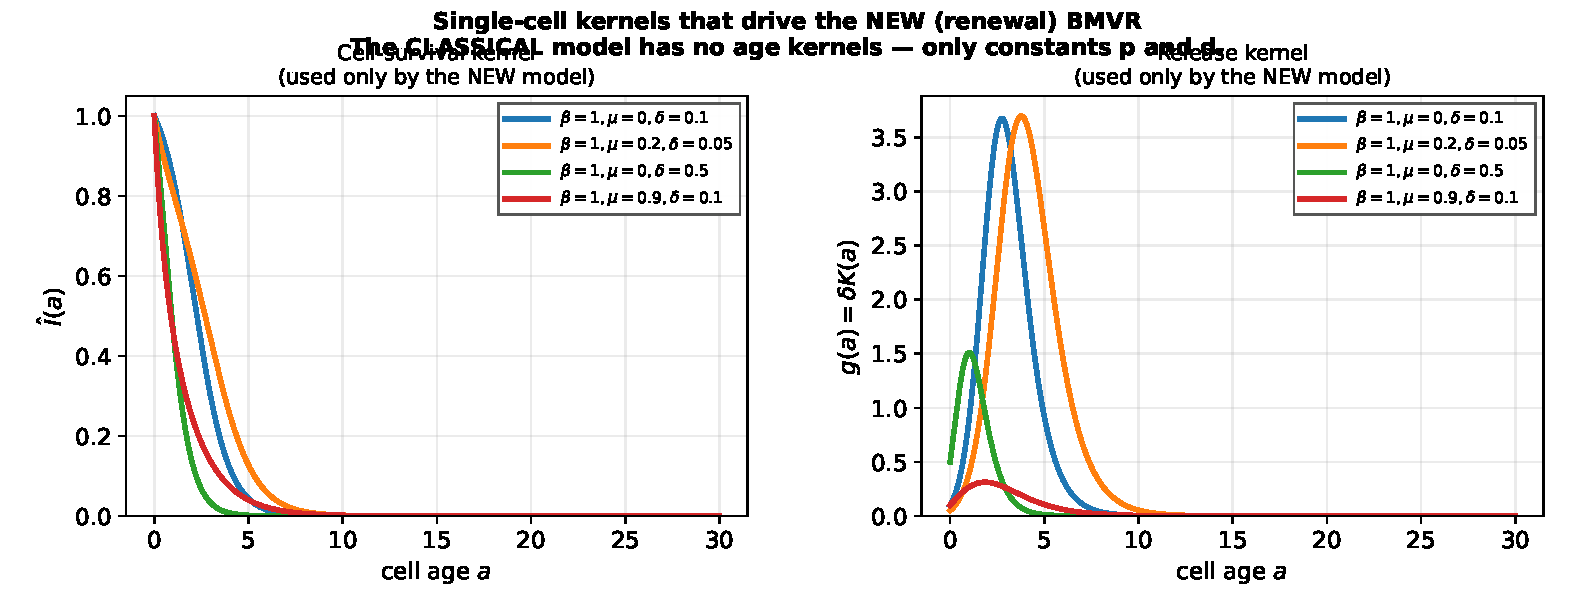
\includegraphics[width=0.86\textwidth]{figures/kernels.pdf}
\caption{The cell-survival kernel $\Ifix(a)$ and the release kernel
$g(a)=\delta K(a)$ for four intracellular parameter sets. These
age-dependent kernels drive the renewal model of this section; the
classical model \eqref{eq:BMVR-classical} has no kernels, only the
constants $p$ and $d_{\Icell}$.}
\label{fig:kernels}
\end{figure}

\subsection{The renewal system}

Hold target cells $T$ fixed, let infection occur at rate $\gamma$ per
virion, clear virions at rate $c$, and define the incidence
\begin{equation}
i(t)=\gamma T\,\Vfree(t).
\end{equation}
Each infection event at time $t-\alpha$ starts a new cell of age $\alpha$;
such a cell is still productive with probability $\Ifix(\alpha)$ and
releases at expected rate $g(\alpha)$. Summing over all infection times,
and adding the contribution $\Icell_0$ of cells already infected at $t=0$,

\figureflag{F4b.1}{Renewal construction schematic}{%
\textbf{Purpose:} the bookkeeping of Result~\ref{res:new-vde} in one
picture: infection events start cohorts, cohorts age, survival and release
are weighted by the two kernels, and the convolutions assemble
$\Icell(t)$ and $\Vfree(t)$. \textbf{Type:} TikZ schematic, inline with
chapter fonts. \textbf{Content:} a horizontal time axis; along it, several
cohort markers at infection times $t-\alpha$ (with $\alpha$ marked as the
age axis running backwards from $t$); each cohort carrying two annotated
weights --- survival $\Ifix(\alpha)$ (a decaying curve sketch) and release
$g(\alpha)=\delta K(\alpha)$ (a curve sketch rising then falling, as in
\Figref{fig:kernels}); arrows from the weighted cohorts into boxes labelled
$\Icell(t)$ (sum of survivors) and $\Vfree'(t)$ (sum of releases, minus
clearance $c\Vfree$); an incidence input arrow labelled $i(t)=\gamma T\Vfree(t)$
closing the loop. \textbf{Labels:} $t$, age $\alpha$, $\Ifix(\alpha)$,
$g(\alpha)$, $i(t)$, $\Icell(t)$, $\Vfree(t)$, convolution signs $*$.
\textbf{Style:} TikZ, inline with chapter fonts, black arrows, the two
kernel curves optionally in colour matching \Figref{fig:kernels}.
\textbf{Placement:} \Secref{sec:renewal}, directly before
Theorem~\ref{res:new-vde}.}

\begin{theorem}[New viral dynamics --- burst-aware BMVR]
\label{res:new-vde}
\begin{equation}
\Icell(t)=\Icell_0\,\Ifix(t)+\int_0^t i(t-\alpha)\,\Ifix(\alpha)\,\dd\alpha
=\Icell_0\,\Ifix+(i*\Ifix)(t),
\label{eq:Icell}
\end{equation}
\begin{equation}
\ddt{\Vfree}(t)
=\Icell_0\,g(t)+\int_0^t i(t-\alpha)\,g(\alpha)\,\dd\alpha-c\,\Vfree(t)
=\Icell_0\,g+(i*g)(t)-c\,\Vfree(t).
\label{eq:Vfree}
\end{equation}
\end{theorem}

\noindent
The correspondence with the classical model is:
\begin{center}
\renewcommand{\arraystretch}{1.3}
\begin{tabular}{@{}p{0.42\textwidth}p{0.48\textwidth}@{}}
\toprule
Classical BMVR \eqref{eq:BMVR-classical} & New system \eqref{eq:Icell}--\eqref{eq:Vfree} \\
\midrule
$\Icell'=i-d_{\Icell}\Icell$
  (constant removal rate $d_{\Icell}$)
& $\Icell = \Icell_0\Ifix + i*\Ifix$
  (age-structured survival via $\Ifix$) \\[0.6em]
$\Vfree'=p\Icell-c\Vfree$
  (constant release rate $p$)
& $\Vfree' = \Icell_0 g + i*g - c\Vfree$
  (age-structured release via $g=\delta K$) \\
\bottomrule
\end{tabular}
\end{center}
Both constant terms are replaced, not just the release: the memoryless
removal $d_{\Icell}\Icell$ becomes the age structure implicit in
\eqref{eq:Icell}, and the constant release $p\Icell$ becomes the
convolution with $g$. A replacement that touched only the release term ---
the natural first thought of \S\ref{sec:proposal-fails} --- would leave the
removal side still memoryless, and still wrong.

Differentiating \eqref{eq:Icell} makes the structure visible:
\begin{equation}
\ddt{\Icell}
= i(t)+\Icell_0\,\Ifix'(t)+\int_0^t i(t-\alpha)\,\Ifix'(\alpha)\,\dd\alpha,
\end{equation}
in which the incidence appears as a source exactly as in the classical
model, while the remaining terms encode age-dependent loss of
productivity. There is, in general, no constant $d_{\Icell}$ for which this
reduces to $\Icell'=i-d_{\Icell}\Icell$ for every history of $i$: such a
reduction holds only when everything grows exponentially, and that exception
is exactly what \S\ref{sec:peff-section} exploits.

\begin{remark}[What is and is not new]
\label{rem:novelty}
The renewal, or age-structured, framework itself is standard: it is the
McKendrick--von Foerster machinery of mathematical demography
\cite{mckendrick1926applications,vonfoerster1959some}, and age-structured
variants of within-host models are well studied. The novelty here is not
the framework. It is that the kernels $\Ifix$ and $g$ are \emph{derived in
closed form from a mechanistic intracellular stochastic process}, rather
than posited phenomenologically --- together with the consequences drawn in
the next three sections. Any honest write-up must say so plainly.
\end{remark}

\subsection{Numerical verification}
\label{sec:renewal-verification}

Result~\ref{res:new-vde} was verified end-to-end by a dedicated numerical
suite (\texttt{verify\_result\_20\_1.py}); the full catalogue is
Appendix~\ref{app:verification}. The tests cover four layers: kernel
integrity (the inputs obey the single-cell identities, five parameter
sets); the $\gamma T=0$ reduction (with no reinfection, \eqref{eq:Icell}--
\eqref{eq:Vfree} collapse to $\Icell=\Icell_0\Ifix$ and the forced linear
equation $\Vfree'=\Icell_0 g-c\Vfree$, matching the single-cell
convolution to machine precision, and with $c=0$ giving
$\Vfree=\Icell_0 V(t)$); structural limits (exponential kernels reproduce
classical BMVR to relative error $<5\times10^{-5}$,
Figure~\ref{fig:D-exp}; the late exponential growth rate equals the
characteristic root $r_*$ of \S\ref{sec:peff-section} to $\sim10^{-7}$,
Figure~\ref{fig:E-growth}; the $R_0$ threshold is sharp,
Figure~\ref{fig:F-R0}); and stochastic ground truth --- an independent
Gillespie ensemble of BDC cells with virion clearance reproduces the
renewal means for $\Icell$ and $\Vfree$ within sampling error
($\gamma T=0$), Figure~\ref{fig:H-gill}. \textbf{Headline: all 54 checks
pass} (the full catalogue, with tallies and reproduction instructions, is
Appendix~\ref{app:verification}).

\begin{figure}[H]
\centering

\includegraphics[width=0.86\textwidth]{figures/D_exponential_reduction.pdf}
\caption{Structural correctness: when the kernels are pure exponentials,
$S=e^{-da}$, $g=p e^{-da}$, the renewal system \eqref{eq:Icell}--
\eqref{eq:Vfree} \emph{is} classical BMVR with those $(p,d)$. Relative
discrepancy $<5\times10^{-5}$ for three matched parameter pairs.}
\label{fig:D-exp}
\end{figure}

\begin{figure}[H]
\centering
\begin{subfigure}{0.47\textwidth}
\centering
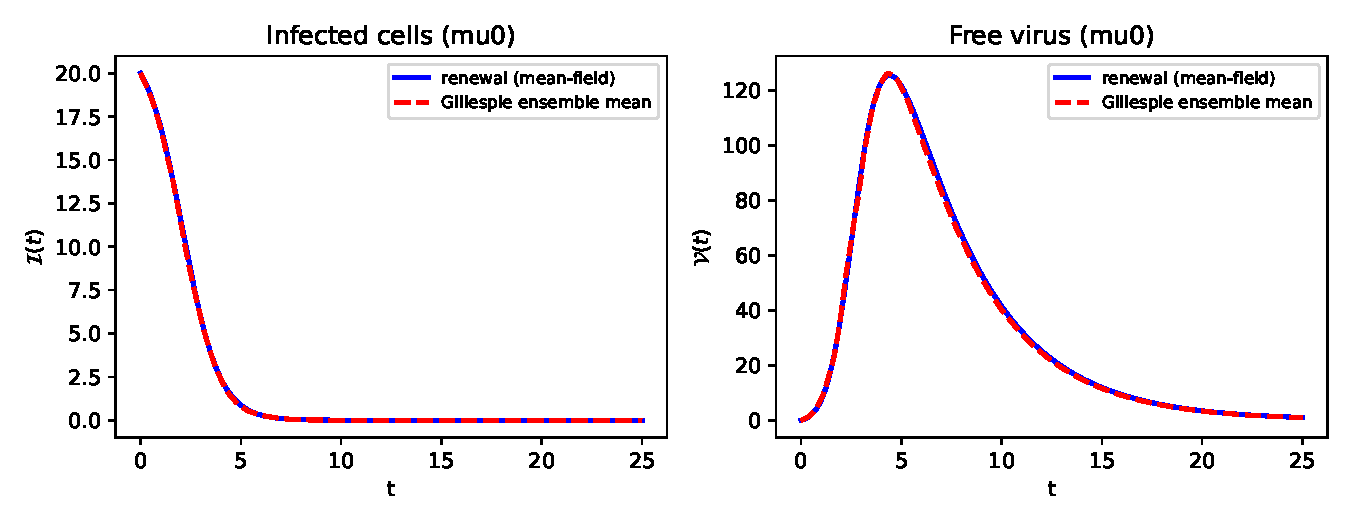
\includegraphics[width=\textwidth]{figures/H_gillespie_mu0.pdf}
\caption{$\mu=0$.}
\end{subfigure}
\hspace{\fill}
\begin{subfigure}{0.47\textwidth}
\centering
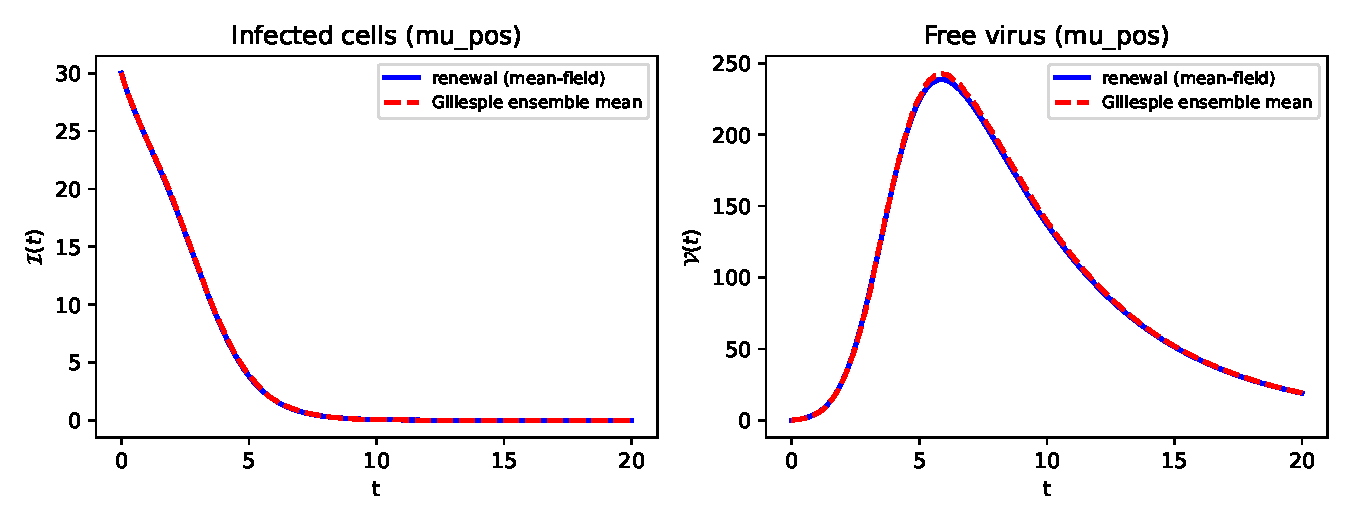
\includegraphics[width=\textwidth]{figures/H_gillespie_mu_pos.pdf}
\caption{$\mu>0$.}
\end{subfigure}
\caption{Stochastic ground truth: ensemble means of an independent Gillespie
simulation of BDC cells (impulse releases at burst times, exponential
clearance, no reinfection) against the renewal solution, relative $L^2$
$\sim1$--$2\%$.}
\label{fig:H-gill}
\end{figure}

\subsection{Overlays: classical vs renewal}
\label{sec:overlays}

To see what age structure does to an epidemic, integrate both systems side
by side. In Figures~\ref{fig:overlay-V}--\ref{fig:growth-phase}, solid navy
is the renewal model \eqref{eq:Icell}--\eqref{eq:Vfree}; dashed orange with
circles is classical BMVR with the fairest constant-parameter match at the
$r=0$ end of the effective-rate map of \S\ref{sec:peff-section},
\begin{equation}
p=p_{\rm eff}(0)=\frac{V_\infty}{\mean{T_{\rm prod}}}
=\frac{\lambda V_\infty}{\log\bigl(a/(a-1)\bigr)},
\qquad
d_{\Icell}=d_{\Icell,{\rm eff}}(0)=\frac{\lambda}{\log\bigl(a/(a-1)\bigr)},
\label{eq:r0match}
\end{equation}
so that total lifetime output and mean productive lifetime agree.

\begin{figure}[H]
\centering

\includegraphics[width=0.86\textwidth]{figures/overlay_V.pdf}
\caption{Free-particle trajectories $\Vfree(t)$. Solid navy: renewal;
dashed orange with circles: classical BMVR matched at $r=0$. Six scenarios:
supercritical growth, subcritical decay, fast burst, high intracellular
death, and free-particle-only seeding.}
\label{fig:overlay-V}
\end{figure}

\begin{figure}[H]
\centering
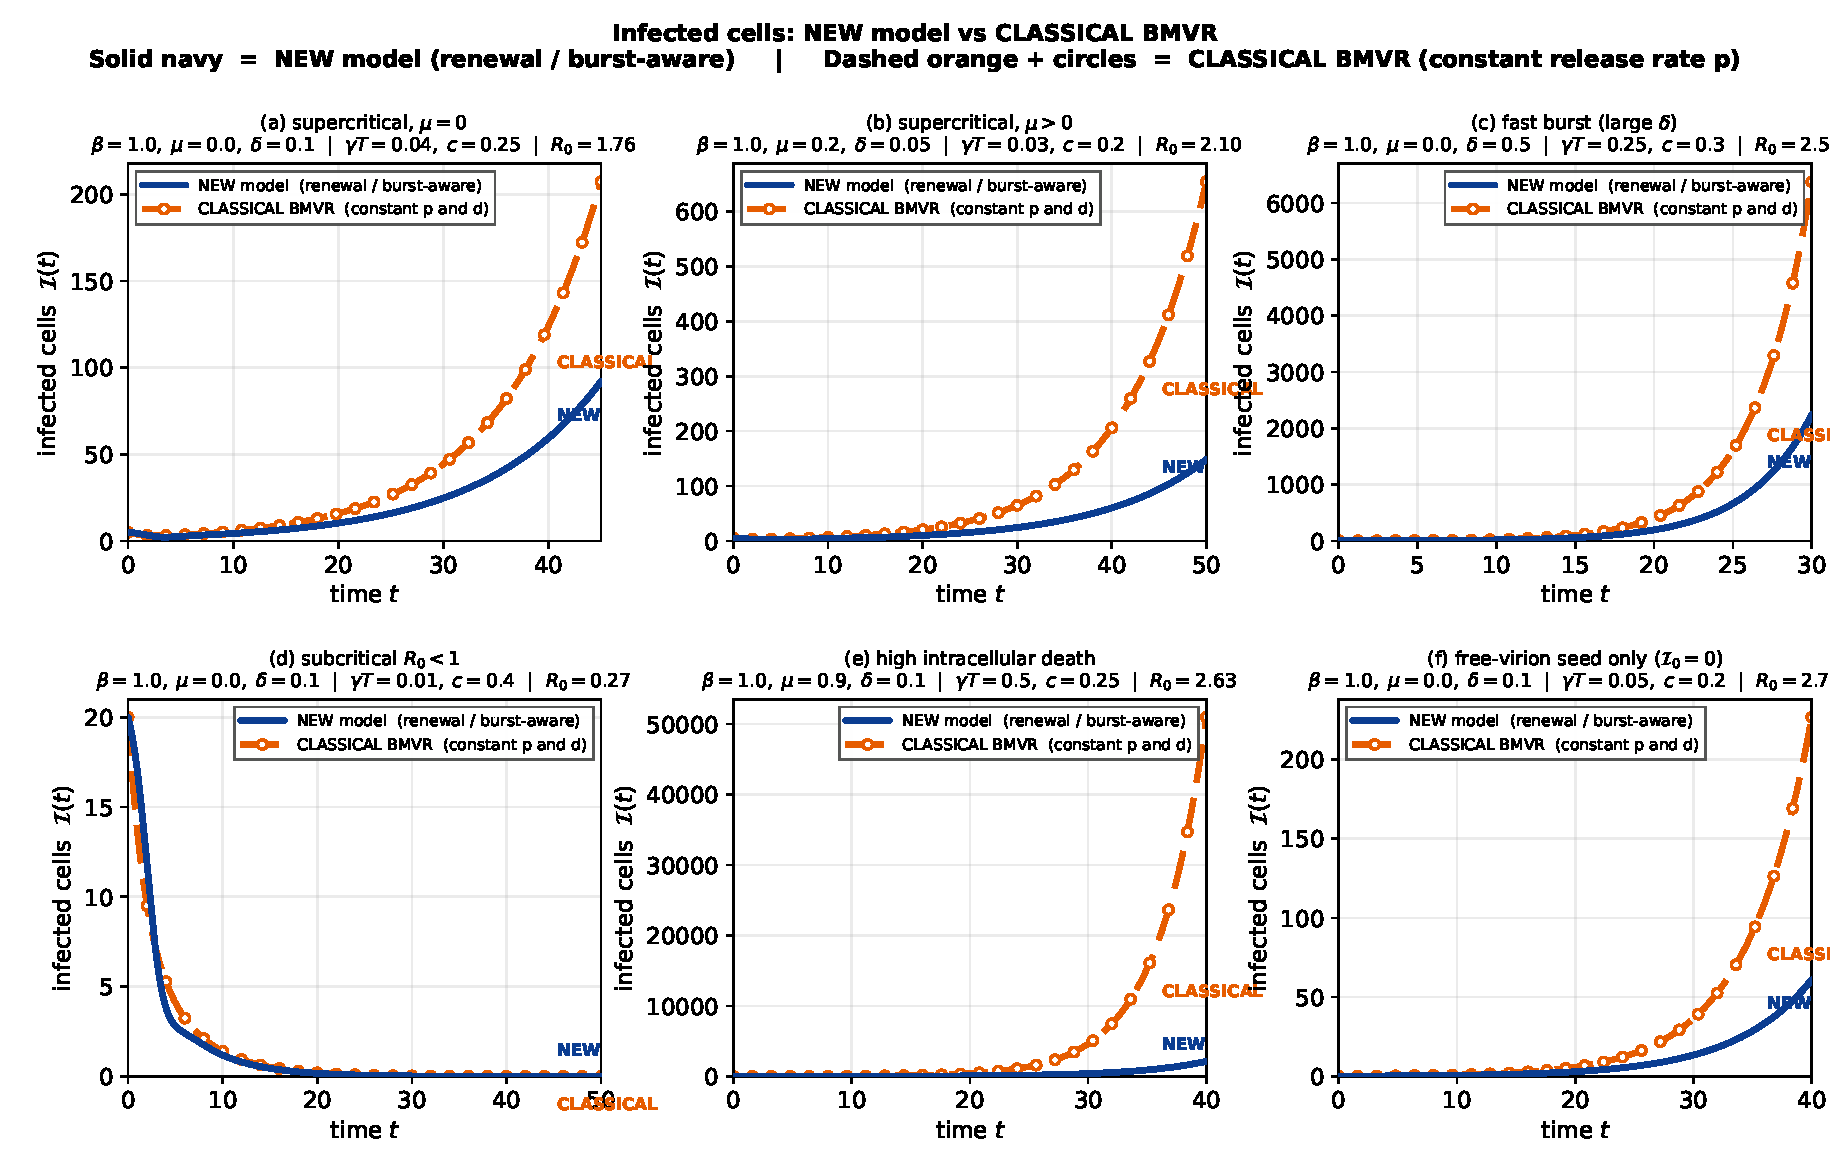
\includegraphics[width=0.86\textwidth]{figures/overlay_I.pdf}
\caption{Infected-cell trajectories $\Icell(t)$ for the same six scenarios;
same line code as Figure~\ref{fig:overlay-V}.}
\label{fig:overlay-I}
\end{figure}

\begin{figure}[H]
\centering

\includegraphics[width=0.86\textwidth]{figures/overlay_V_with_naive.pdf}
\caption{The naive proposal \eqref{eq:naive-p} as a third curve (dotted
green): classical BMVR with $p=\langle X\rangle_{\rm QS}$ --- a count used
as a rate --- is systematically wrong in scale, not merely in shape.}
\label{fig:overlay-V-naive}
\end{figure}

The reading is consistent across panels. The matched classical model often
gets the order of magnitude but not the shape: it misses the early lag
(young cells dominate, and release is closer to the young-cell limit
$p\to\delta$ than to $p_{\rm eff}(0)$), the timing of the peak, and the
late growth rate (as the epidemic grows, generation-time structure moves
the operative release rate away from its $r=0$ value). The relative
free-particle discrepancy,
\begin{equation}
\frac{\bigl|\Vfree^{\rm new}(t)-\Vfree^{\rm classical}(t)\bigr|}
{\max_s \Vfree^{\rm new}(s)},
\end{equation}
is often order one or larger by the end of the plotted window in
supercritical regimes, and is worst when intracellular death is high
(Figure~\ref{fig:rel-diff}): there, $V_\infty$ is small while the
age-structure of release remains strongly non-exponential. Discrepancies
grow with $R_0$ and with the strength of age-structure in the kernels
(slow bursting, non-zero $\mu$).

\begin{figure}[H]
\centering

\includegraphics[width=0.86\textwidth]{figures/overlay_rel_diff.pdf}
\caption{Relative free-particle discrepancy between the renewal model and
matched classical BMVR across the six scenarios. Large values mean the
constant-$p$ ODEs fail to track the burst-aware model.}
\label{fig:rel-diff}
\end{figure}

\begin{figure}[H]
\centering

\includegraphics[width=0.86\textwidth]{figures/overlay_growth_phase.pdf}
\caption{Growth-phase mismatch for one supercritical set
($\lambda=1$, $\mu=0$, $\delta=0.1$). Solid navy: renewal; dashed orange:
classical matched at $r=0$; dash-dot purple: classical with the young-cell
parameters $p=\delta$, $d_{\Icell}=\mu+\delta$. Neither classical choice
tracks the renewal curve across the whole trajectory --- the $r=0$ match
fails early, the young-cell match fails late. Left panel logarithmic in
$\Vfree$.}
\label{fig:growth-phase}
\end{figure}

These numerical facts are exactly what the analytic reduction of the next
section predicts: a constant pair $(p,d_{\Icell})$ can reproduce one
exponential growth rate exactly, but not a transient that samples a
continuum of cell ages.
